%%%%%%%%%%%%%%%%%%%%%%%%%%%%%%%%%%%%%%%%%%%%%%%%%%%%%%%%%%%
% --------------------------------------------------------
% Tau
% LaTeX Template
% Version 2.4.4 (28/02/2025)
%
% Author: 
% Guillermo Jimenez (memo.notess1@gmail.com)
% 
% License:
% Creative Commons CC BY 4.0
% --------------------------------------------------------
%%%%%%%%%%%%%%%%%%%%%%%%%%%%%%%%%%%%%%%%%%%%%%%%%%%%%%%%%%%

\documentclass[9pt,a4paper,twocolumn,twoside]{tau-class/tau}
\usepackage[english]{babel}

%% Draft watermark
% \usepackage{draftwatermark}

\usepackage{pdfpages}

%----------------------------------------------------------
% TITLE
%----------------------------------------------------------

\journalname{M.Sc. Physics: Spectroscopy}
\title{Second- and Third-Harmonic Generation}

%----------------------------------------------------------
% AUTHORS, AFFILIATIONS AND PROFESSOR
%----------------------------------------------------------

\author[a,1]{Florian Marius Adamczyk}

%----------------------------------------------------------

\affil[a]{Justus-Liebig-Universität Gießen, Institute of Physics, Germany}

\professor{PD Dr. Arash Rahimi-Iman, Dipl.-Ing.}

%----------------------------------------------------------
% FOOTER INFORMATION
%----------------------------------------------------------

\institution{Justus-Liebig-Universität Gießen}
\footinfo{SHG \& THG Report}
\theday{\today}
\leadauthor{Adamczyk, F.}
\course{M.Sc. Physics: Spectroscopy}

%----------------------------------------------------------
% ABSTRACT AND KEYWORDS
%----------------------------------------------------------

\begin{abstract}    
    In this report, we explore the fundamentals of second- and third-harmonic generation,
    focusing on how nonlinear polarization leads to frequency doubling and tripling of light.
    We discuss phase-matching strategies and practical considerations, showcasing how SHG and THG
    drive innovations in ultrafast lasers, microscopy, and material characterization.
\end{abstract}

%----------------------------------------------------------

\keywords{SHG, THG, Nonlinear Optics, Phase Matching}

%----------------------------------------------------------

\begin{document}
		
    \maketitle 
    \thispagestyle{firststyle} 
    \tauabstract 
    % \tableofcontents
    % \linenumbers 
    
%----------------------------------------------------------

\section{Introduction \& Motivation}
    \taustart{N}onlinear optical processes extend linear spectroscopy by enabling frequency conversion through intense electromagnetic fields interacting with matter. In particular, \emph{second-harmonic generation} (SHG) and \emph{third-harmonic generation} (THG) provide access to new spectral regions and high-resolution imaging capabilities. Applications include ultrafast laser pulse characterization, biological microscopy, and material property analysis.

\section{Fundamentals of Nonlinear Polarization}
The response of a dielectric medium to an applied electric field $E(t)$ can be expanded as:
\begin{equation}
P(t) = \varepsilon_0\bigl[\chi^{(1)}E(t) + \chi^{(2)}E^2(t) + \chi^{(3)}E^3(t) + \cdots\bigr],
\end{equation}
where $\chi^{(n)}$ denotes the $n$th-order nonlinear susceptibility tensor. The second-order term gives rise to SHG, generating polarization oscillating at $2\omega$, whereas the third-order term produces THG at $3\omega$ and other phenomena such as four-wave mixing.

\subsection{Energy and Momentum Conservation}
Efficient harmonic generation requires satisfaction of conservation laws:
\begin{description}
    \item[Energy conservation:] \hspace{0.5em} $\displaystyle \sum_i \hbar \omega_i = \hbar n\omega$
    \item[Momentum conservation (phase matching):] \hspace{0.5em} $\displaystyle \sum_i \vec{k}_i = n\vec{k}(\omega)$
\end{description}
Here, $\vec{k}(\omega)$ is the wavevector at frequency $\omega$. For efficient conversion, the phase mismatch $\Delta k = n k(\omega) - \sum_i k_i$ should vanish.

\section{Second-Harmonic Generation (SHG)}
SHG arises in noncentrosymmetric crystals through the second-order polarization:
\begin{equation}
P_i(2\omega) = \varepsilon_0 \sum_{jk} \chi^{(2)}{ijk} E_j(\omega)E_k(\omega).
\end{equation}

\begin{figure}[!ht] % Adjusted float specifier
\centering
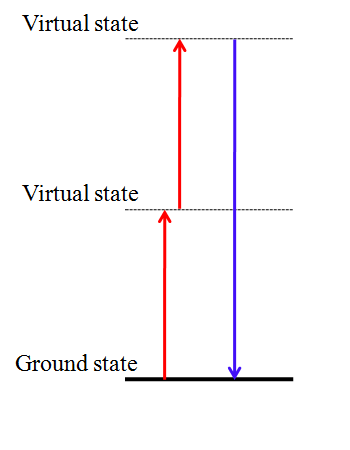
\includegraphics[width=0.35\columnwidth]{figures/Energy_level_scheme_of_SHG.png}
\caption{Energy level scheme of SHG process. \cite{SobarwikiImage} The fundamental frequency $\omega$ is converted to the second harmonic $2\omega$.}
\end{figure}

\subsection{Tensor Properties}
The $\chi^{(2)}{ijk}$ tensor has specific nonzero components determined by crystal symmetry. For example, in a LiNbO$3$ crystal:
\begin{table}[h!]
\centering
\begin{tabular}{l c}
\toprule
Component & Value (pm/V) \\
\midrule
$d_{31} = \chi^{(2)}_{311}$ & 4.5 \\
$d_{33} = \chi^{(2)}_{333}$ & 27.0 \\
\bottomrule
\end{tabular}
\caption{Selected nonlinear coefficients for LiNbO$_3$.}
\end{table}

\subsection{Phase-Matching Techniques}
\textbf{Birefringent Phase Matching.} By exploiting crystal birefringence, one can choose ordinary and extraordinary polarizations to satisfy:
\begin{equation}
n k_o(\omega) = k_e(2\omega).
\end{equation}
\textbf{Quasi-Phase Matching.} Periodic poling in materials such as PPLN introduces a modulation of $\chi^{(2)}$ with period $\Lambda$, compensating phase mismatch via reciprocal vectors $G = 2\pi/\Lambda$.

\begin{figure}[!ht] % Adjusted float specifier
\centering
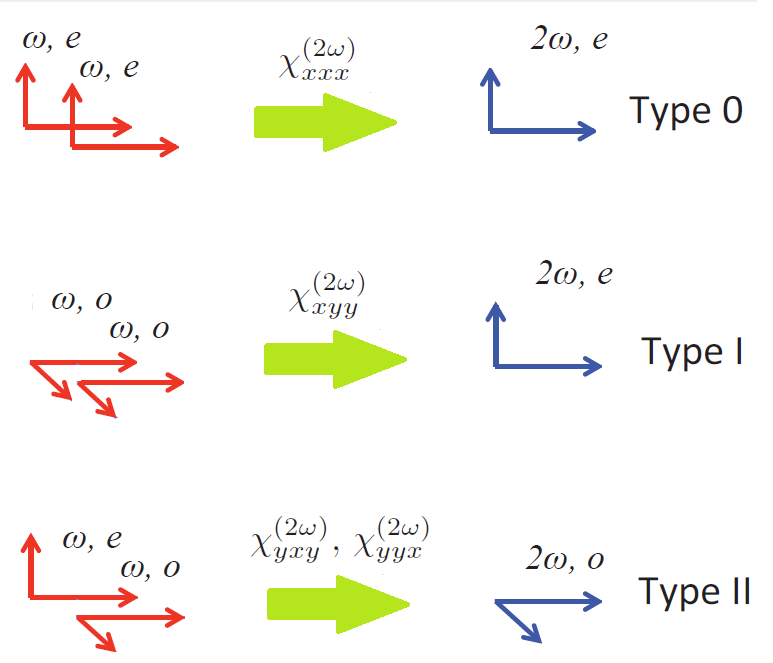
\includegraphics[width=0.7\columnwidth]{figures/TypeX_SHG.png}
\caption{Different types of second-harmonic generation phase-matching of a coherent light for strong conversion. The case of negative crystals ($n_o > n_e$) is considered; invert indices if positive crystal ($n_e > n_o$). \cite{PhasemathingImage}}
\end{figure}

\section{Third-Harmonic Generation (THG)}
THG is a third-order process present in both centrosymmetric and noncentrosymmetric media, described by:
\begin{equation}
P_i(3\omega) = \varepsilon_0 \sum_{jkl} \chi^{(3)}_{ijkl} E_j(\omega)E_k(\omega)E_l(\omega).
\end{equation}

\subsection{Phase Matching and Cascading}
Perfect phase matching for THG is challenging; one may use
\begin{itemize}
\item \emph{Bulk phase matching}, adjusting dispersion via angle or temperature tuning.
\item \emph{Cascading SHG processes}, where sequential $\chi^{(2)}$ interactions ($\omega \to 2\omega$, then $\omega+2\omega \to 3\omega$) effectively generate THG with enhanced efficiency.
\end{itemize}

% \begin{figure}[h!]
% \centering
% \includegraphics[width=0.6\textwidth]{thg_cascading.png}
% \caption{Energy-level diagram illustrating cascaded SHG and sum-frequency mixing to produce THG.}
% \end{figure}

\section{Historical Perspective on SHG}
Second-harmonic generation (SHG) has a rich history closely tied to the development of laser technology. Key milestones include:

\begin{itemize}
    \item \textbf{1961: Experimental Breakthrough} \\
    At the University of Michigan, Peter Franken, A. E. Hill, C. W. Peters, and G. Weinreich demonstrated SHG by focusing a ruby laser (694 nm) into a quartz sample and observing light at 347 nm (frequency doubling). Notably, a copy editor once mistakenly removed the dim 347 nm spot from the published figures in Physical Review Letters.
    
    \item \textbf{1962: Theoretical Framework} \\
    N. Bloembergen and P. S. Pershan at Harvard provided a formal theoretical description of SHG. By analyzing Maxwell's equations at the interface between linear and nonlinear media, they established the fundamental rules governing light interactions in nonlinear systems, laying the groundwork for the rapid expansion of nonlinear optics.
\end{itemize}

\section{Experimental Setup and Considerations}
A typical setup for SHG/THG experiments includes:
\begin{itemize}
\item A femtosecond pulsed laser (e.g., Ti:sapphire, 800nm, 100fs)
\item Beam-shaping and focusing optics (lenses or microscope objectives)
\item Nonlinear crystal mounted on a rotation/temperature-controlled stage
\item Filters or dichroic mirrors to separate fundamental and harmonic beams
\end{itemize}

\begin{figure}[!ht] % Adjusted float specifier
\centering
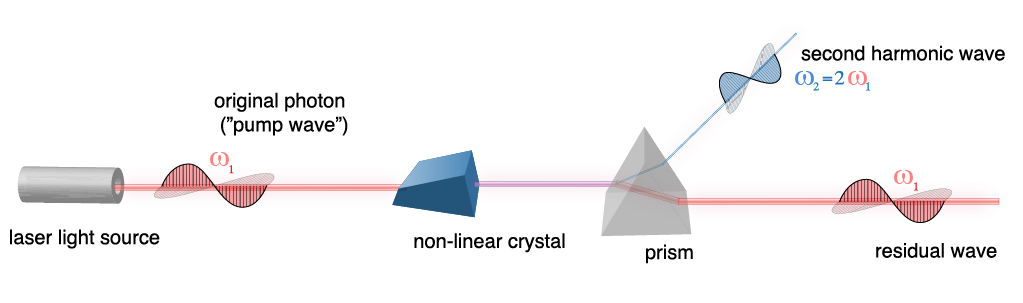
\includegraphics[width=0.95\columnwidth]{figures/experimental.png}
\caption{Schematic of a typical experimental setup for SHG and THG. A femtosecond laser is focused onto a nonlinear crystal, and generated harmonics are separated from the fundamental using dichroic mirrors and filters. \cite{JkwchuiImage}}
\end{figure}

Key challenges include crystal damage thresholds, beam walk-off, and maintaining spatial overlap. Temperature stabilization is often required for fine-tuning phase matching.

\section{Applications}
\subsection{SHG Microscopy}
SHG microscopy leverages noncentrosymmetric structures (e.g., collagen, myosin) to provide label-free imaging in biology. The nonlinear effect offers high spatial resolution and intrinsic contrast without external dyes. This technique is particularly useful for probing ordered tissues, mapping structural proteins, and investigating dynamic processes in living organisms.

\subsection{SHG from Planar Surfaces}
\textbf{Surface Second-Harmonic Generation.} SHG has been extensively used to study molecular orientation and ordering at planar interfaces, such as the air-water boundary. Early experiments demonstrated SHG from metal surfaces, but its application to liquid interfaces provided groundbreaking insights into molecular behavior at ubiquitous surfaces.

The specific elements of the second-order susceptibility tensor $\chi^{(2)}$ can be expressed as:
\begin{align}
\chi_{zzz}^{(2)} &= N_s \langle \cos^3(\theta) \rangle \alpha_{zzz}^{(2)}, \\
\chi_{xzx}^{(2)} &= \frac{1}{2} N_s \langle \cos(\theta) \sin^2(\theta) \rangle \alpha_{zzz}^{(2)},
\end{align}
where $N_s$ is the adsorbate density, $\theta$ is the angle between the molecular axis $z$ and the surface normal $Z$, and $\alpha_{zzz}^{(2)}$ is the dominant nonlinear polarizability element of a molecule at the interface. \cite{SecondHarmonicGeneration}

Using interference SHG methods, these tensor elements can be determined, enabling the measurement of molecular orientation. For example, studies of phenol at the air-water interface revealed that the hydroxyl group points downward into the water, consistent with its hydrogen-bonding potential. SHG has also uncovered differences in $pK_a$ values and rotational dynamics of molecules at interfaces.

\begin{figure}[h!]
\centering
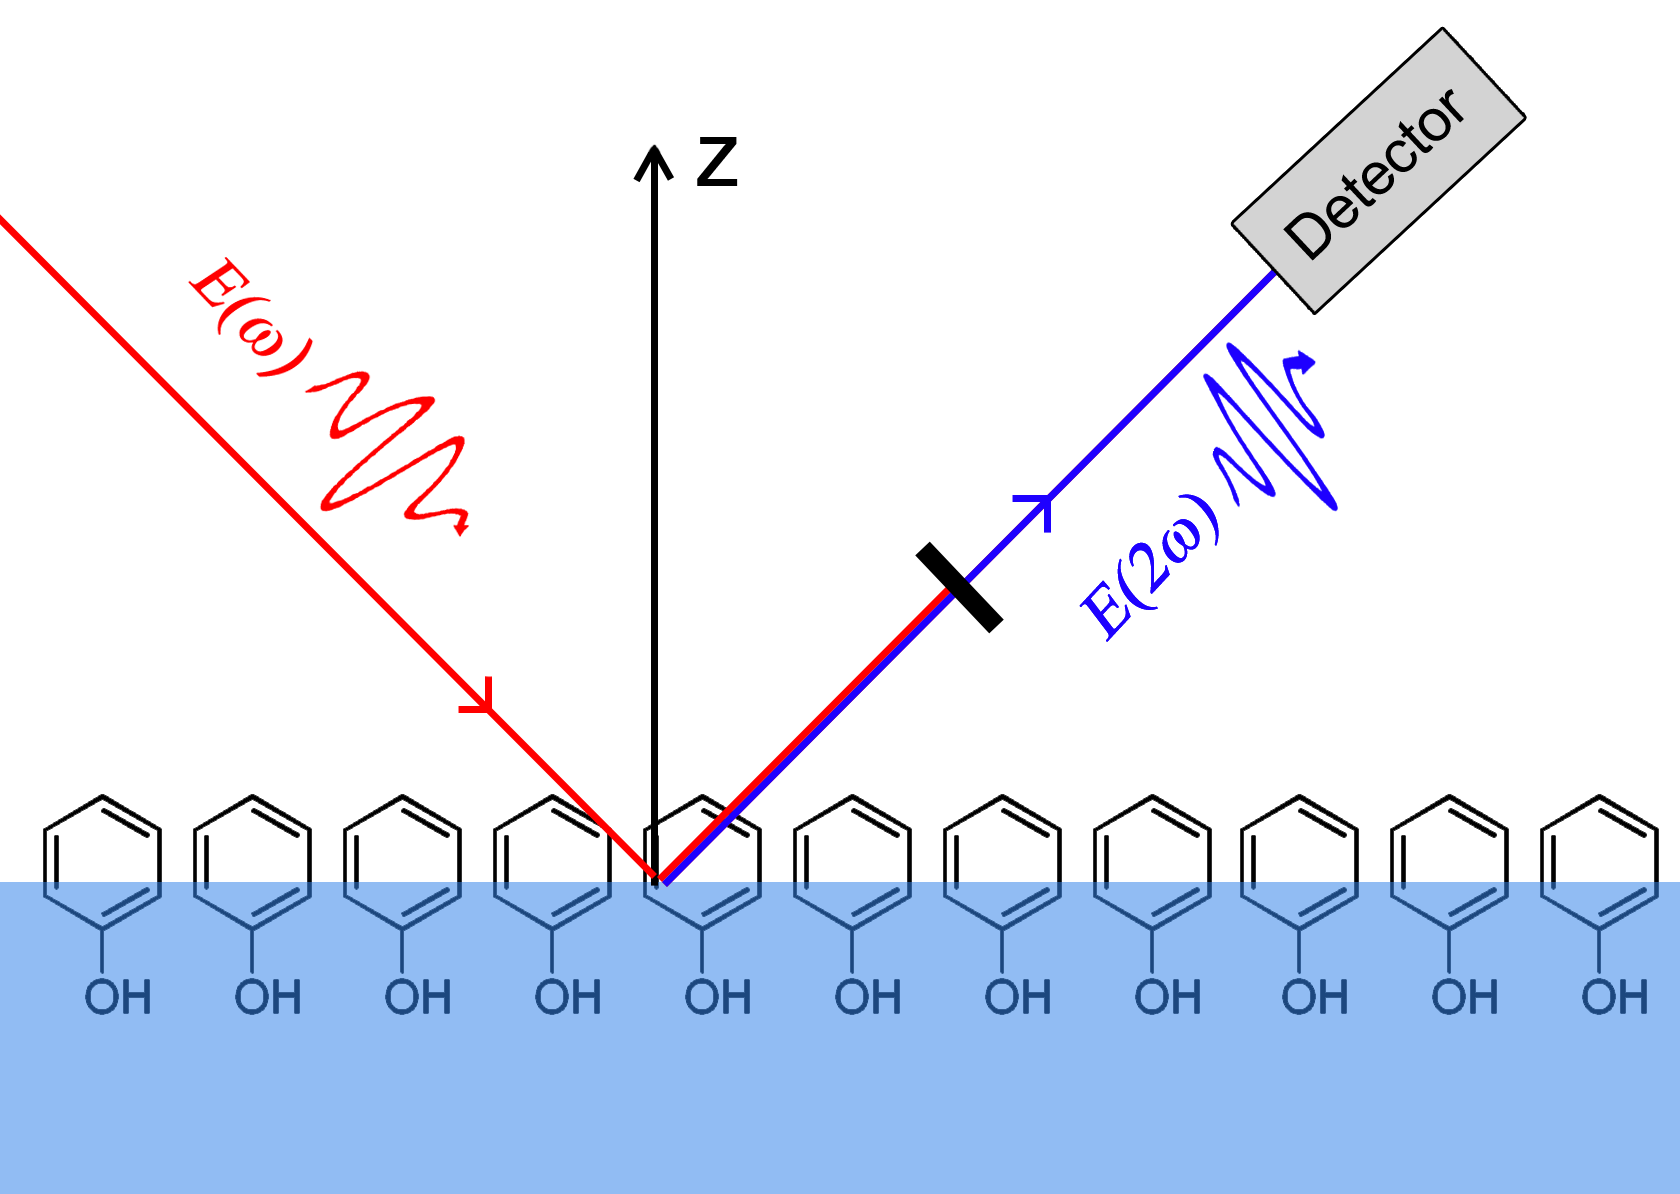
\includegraphics[width=0.7\columnwidth]{figures/SHG_phenol_air-water.png}
\caption{SHG setup for measuring the orientation of phenol at the air-water interface. The technique provides detailed information about molecular orientation and ordering at planar surfaces.\cite{Swk2118Image}}
\end{figure}

\subsection{Ultraviolet THG Spectroscopy}
Tripling near-infrared laser light generates coherent UV signals for high-resolution absorption measurements. This approach is valuable for characterizing electronic transitions, studying photonic materials, and probing thin films. By tuning the fundamental wavelength and using angle-phase-matching conditions, tunable UV beams enable detailed investigations into band structures and excitonic resonances.

\section{Summary and Outlook}
We have reviewed the physical principles of SHG and THG, emphasizing the roles of $\chi^{(2)}$ and $\chi^{(3)}$ susceptibilities and phase-matching strategies. Future directions include integrated photonic waveguides with engineered dispersion and metasurfaces for enhanced harmonic conversion efficiencies.
	
    

%----------------------------------------------------------

\printbibliography % Ensure bibliography is printed

%----------------------------------------------------------

\section*{Appendix}
In the following appendix, I included some conversations with LLMs used to create this report.


\includepdf[pages=-]{LLM_documentation/001.pdf}
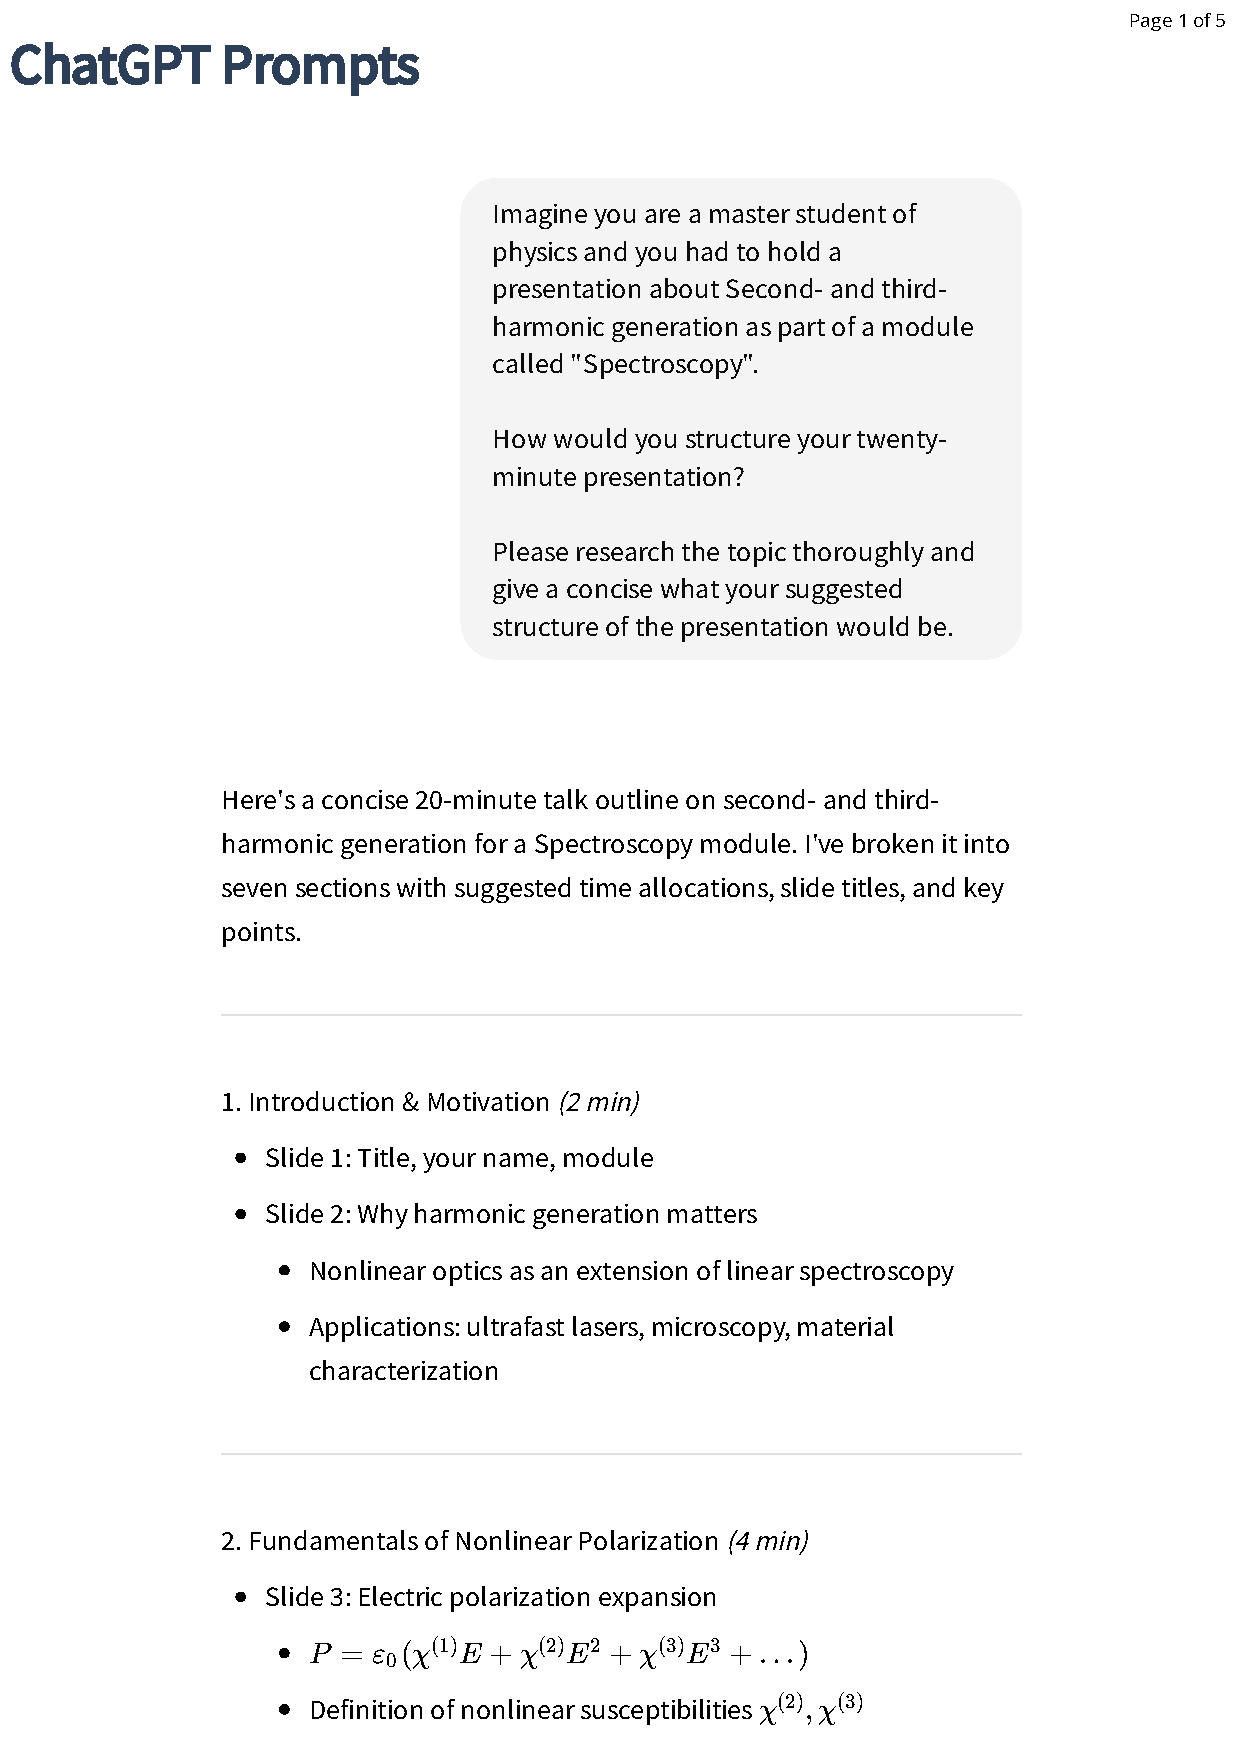
\includepdf[pages=-]{LLM_documentation/+01.pdf}
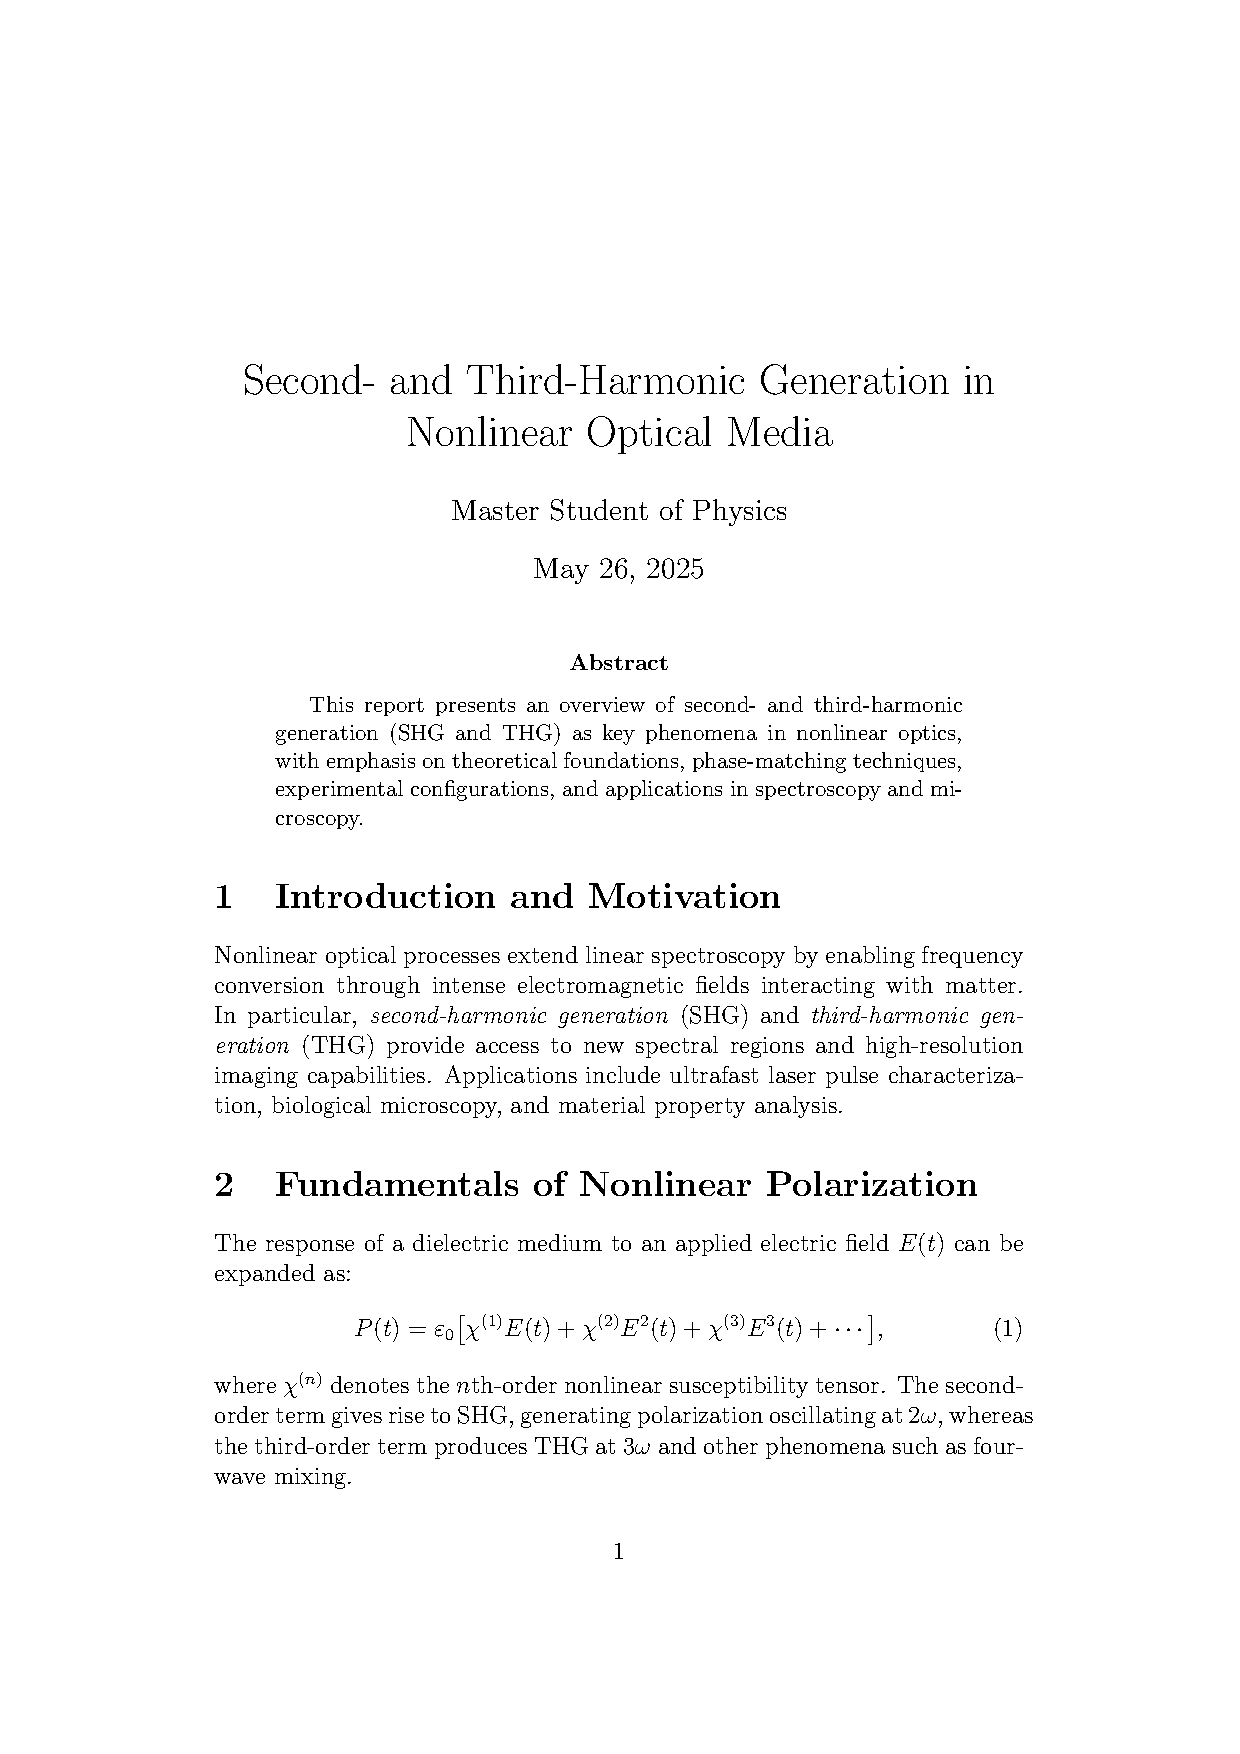
\includepdf[pages=-]{LLM_documentation/FirstTest/firstTest.pdf}


\end{document}